\chapter{Relazioni Ricorsive}

\begin{flushleft}
    Una successione $\{a_n\}_{n \in \mathbb{N}}$ a valori interi può essere data in due forme differenti:
    \begin{itemize}[nosep]
        \item per \textbf{elencazione}: $\{a_0, a_1, ..., a_i, ...\}$, con $a_i \in mathbb{Z} \; \forall i \in \mathbb{N}_0$
        \item in \textbf{forma chiusa}: $a_n = f(n)$, con $f : \mathbb{N}_0 \mapsto \mathbb{Z}$, $f$ è un'\textbf{applicazione}
    \end{itemize}

    \textbf{Successioni Definite per Ricorsione}: una successione è definita \textbf{ricorsivamente} (ovvero tramite una \textbf{relazione ricorsiva}) se ogni termine della successione è espresso in funzione dei termini precedenti, e se sono noti un certo numero di termini iniziali che permettano di individuare univocamente la successione.

    Risolvere una \textit{relazione ricorsiva} significa ottenere una definizione in forma chiusa della successione stessa.

    \begin{boxA}
        \textcolor{orange}{\textbf{Esempio}} \\
        $\begin{cases}
            a_n = 3 \cdot a_{n - 1} \quad n > 1 \; \text{(relazione ricorsiva)} \\
            a_1 = 3 \qquad \qquad \qquad \;\; \text{(condizione iniziale)}
        \end{cases}$ \\
        definisce univocamente la successione \fcolorbox{orange}{white}{$\{a_n\}_{n \in \mathbb{N}} = \{3, 3^2, 3^3, ...\}$} che si può rappresentare in forma chiusa come:

        {\centering
            $a_n = 3^n \; \forall n \in \mathbb{N}$
        \par}
    \end{boxA}

    Una relazione ricorsiva si dice di \textbf{ordine \textit{k}} se il generico elemento $a_n$ della successione è dato in funzione di $k$ elementi che lo precedono. La relazione ricorsiva determinerà univocamente una successione, noti i $k$ elementi iniziali della successione

    Una relazione ricorsiva di ordine $k$ si dice \textbf{lineare} se viene rappresentata come:

    {\centering
        $a_n = b_{n - 1}(n) \cdot a_{n - 1} + b_{n - 2}(n) \cdot a_{n - 2} + ... + b_{n - k}(n) \cdot a_{n - k} + d(n)$
    \par}
    dove i $b_{n - i}(n) \; i \in \mathbb{N}$ sono delle funzioni (non necessariamente lineari) che determinano i coefficienti $a_{n - i} \; i \in \mathbb{N}$ mentre $d(n)$ è il termine noto (può non essere lineare).

    Una relazione ricorsiva \textit{lineare} si dice \textbf{omogenea} se il termine noto è nullo, ovvero $d(n) = 0$

    Una relazione ricorsiva \textit{lineare} si dice a \textbf{coefficienti costanti} se le funzioni coefficienti [$b_{n - i}(n) \; i \in \mathbb{N}$] sono funzioni costanti, ovvero $b_{n - i}(n) = \alpha_i$, con $\alpha_i$ costante $\forall i$ e viene rappresentata:

    {\centering
        $a_n = \alpha_1 \cdot a_{n - 1} + \alpha_2 \cdot a_{n - 2} + ... + \alpha_k \cdot a_{n - k} + d(n)$
    \par}
\end{flushleft}

\section{Relazioni Ricorsive Lineari del 1$^\circ$ Ordine}

\begin{flushleft}
    \textbf{Relazioni ricorsive lineari omogenee del I ordine a coefficienti costanti}: la successione definita da: 

    {\centering
        $\begin{cases}
            a_n = b \cdot a_{n - 1} \quad \forall n > m \\
            a_m = c
        \end{cases}$
    \par}
    ha come forma chiusa: \fcolorbox{red}{white}{$a_n = c \cdot b^{n - m} \; \forall n \geq m$}

    \begin{boxA}
        \textcolor{olive}{\textbf{Dimostrazione}}: si dimostra per \textbf{induzione} \newline
        \textcolor{red}{\textbf{Passo Iniziale}}: poniamo $n = m$ allora avremo che: 

        {\centering
            $a_n = c \cdot b^{m - m} = c \cdot b^0 = c$
        \par}
        abbiamo dimostrato le condizioni di partenza della relazione ricorsiva.

        \textcolor{red}{\textbf{Passo Induttivo}}

        {\centering
            \begin{minipage}[t]{0.45\textwidth}
                \centering
                \textbf{Hp.} $a_{n - 1} = c \cdot b^{n - 1 - m}$
            \end{minipage}
            \begin{minipage}[t]{0.45\textwidth}
                \centering
                \textbf{Th.} $a_n = c \cdot b^{n - m}$
            \end{minipage}
            $a_n = b \cdot a_{n - 1} = b \cdot c \cdot b^{n - 1 - m} = c \cdot b^{n - m}$
        \par}

        \textcolor{orange}{\textbf{Esempio}}

        {\centering
            $\begin{cases}
                a_n = 3a_{a - 1} \\
                a_0 = 2
            \end{cases}$
            $\Rightarrow a_n = 2 \cdot 3^{n - 0} = 2 \cdot 3^n$
        \par}
    \end{boxA}
    \textbf{Relazioni ricorsive lineari omogenee del I ordine a coefficienti non costanti}: la successione definita da:

    {\centering
        $\begin{cases}
            a_n = b(n) \cdot a_{n - 1} \quad \forall n > m \\
            a_m = c
        \end{cases}$
    \par}
    ha come forma chiusa \fcolorbox{red}{white}{$a_n = c \cdot \underset{i = 1}{\overset{n - m}{\prod}} b (m + i) \; \forall n \geq m$}. La forma chiusa può essere dimostrata per \textbf{induzione}, in perfetta analogia al caso precedente:
\end{flushleft}

\newpage
\begin{flushleft}

    \textbf{Relazioni ricorsive lineari del I ordine non omogenee a coefficienti costanti}: la successione definita da:

    {\centering
        $\begin{cases}
            a_n = b \cdot a_{n-1} + d(n) \quad \forall n > m \\
            a_m = c
        \end{cases}$
    \par}
    ha come forma chiusa: \fcolorbox{red}{white}{$a_n = b^{n-m} \cdot [c + \underset{i = 1}{\overset{n-m}{\sum}} d(m + i) \cdot b^{-i}] \; \forall n \geq m$}

    \begin{boxA}
        \textcolor{olive}{\textbf{Dimostrazione}}: la forma chiusa viene dimostrata sempre per \textbf{induzione}

        \textcolor{red}{\textbf{Passo Iniziale}}: poniamo $n = m$

        {\centering
            $a_n = b^{m-m} \cdot [c + \underset{i = 1}{\overset{m-m}{\sum}} d(m + i) \cdot b^{-i}] = [c + \cancel{\underset{i = 1}{\overset{0}{\sum}} d(m + i) \cdot b^{-1}}] = c$
        \par}

        \textcolor{red}{\textbf{Passo Induttivo}}

        {\centering
            \begin{minipage}[t]{0.45\textwidth}
                \centering
                \textbf{Hp.} \\
                $a_{n - 1} = b^{n-1-m} \cdot [c + \underset{i=1}{\overset{n-1-m}{\sum}} d(m + i) \cdot b^{-i}]$
            \end{minipage}
            \begin{minipage}[t]{0.45\textwidth}
                \centering
                \textbf{Th.} \\
                $a_n = b^{n-m} \cdot [c + \underset{i = 1}{\overset{n-m}{\sum}} d(m + i) \cdot b^{-i}]$
            \end{minipage}
        \par}

        $a_n = b \cdot a_{n-1} + d(n) = b \cdot b^{n-1-m} [c + \underset{i=1}{\overset{n-1-m}{\sum}} d(m+i) \cdot b^{-1}] + d(n) \cdot \fcolorbox{brown}{white}{$(b^{n-m} \cdot b^{-(n-m)})$}$ moltiplico e divido per $b^{n-m}$ in modo da poter raccogliere al primo addendo.
        \begin{align*}
            a_n &= b \cdot b^{n-1-m} [c + \underset{i=1}{\overset{n-1-m}{\sum}} d(m+i) \cdot b^{-1}] + d(n) \cdot (b^{n-m} \cdot b^{-(n-m)}) \\
            &= b^{n-m} [c + \underset{i=1}{\overset{n-1-m}{\sum}} d(m+i) \cdot b^{-1}] + d(n) \cdot (b^{n-m} \cdot b^{-(n-m)}) \\
            &= b^{n-m} \cdot \{[c + \underset{i=1}{\overset{n-1-m}{\sum}} d(m+i) \cdot b^{-1}] + \fcolorbox{blue}{white}{$d(n) \cdot b^{-(n-m)}$}\} \\
            &= b^{n-m} \cdot [c + \underset{i = 1}{\overset{n-m}{\sum}} d(m + i) \cdot b^{-i}]
        \end{align*}
        Il valore \fcolorbox{blue}{white}{$d(n) \cdot b^{-(n-m)}$} posso portarlo dentro alla sommatoria in modo da poter ottenere e dimostrare la tesi.
    \end{boxA}
\end{flushleft}

\begin{boxA}
    \textcolor{orange}{\textbf{Esempio - Torre di Hanoi}}: bisogna spostare $n$ dischi di diametro crescente, in modo da riottenere la torre sull'ultima colonna. \textbf{Regole}: ad ogni passo si può spostare un solo disco, un disco non può mai essere spostato sopra ad uno di diametro inferiore.
    
    \begin{center}
        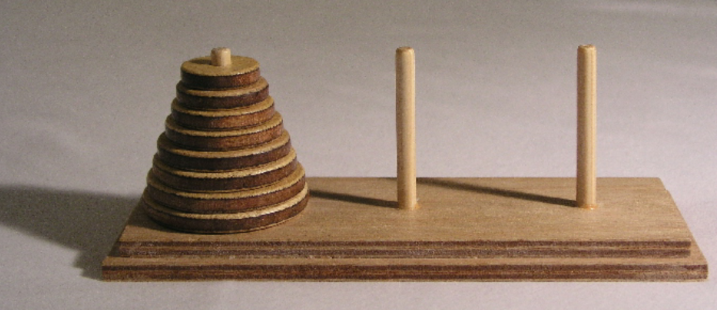
\includegraphics[width=0.65\textwidth]{img/hanoi}
    \end{center}

    Per spostare il generico $n$-esimo disco: $H_n = H_{n-1} + 1 + H_{n-1} = 2 \cdot H_{n-1} + 1$. Quindi la nostra relazione ricorsiva sarà:
    $H(n) = \begin{cases}
        H_n = 2 \cdot H_{n-1} + 1 \\
        H_1 = 1
    \end{cases}$
    
    \begin{align*}
        H(n) &= 2^{n-1} [1 + \underset{i=1}{\overset{n-1}{\sum}}1 \cdot 2^{-i}] \\
        &= 2^{n-1} [\underset{i=0}{\overset{n-1}{\sum}}1 \cdot 2^{-i}] \\
        &= 2^{n-1} \cdot \frac{1-(\frac{1}{2})^n}{1-\frac{1}{2}} \\
        &= 2^n \cdot (1 - \frac{1}{2^n}) = 2^n - 1 \; \text{mosse}
    \end{align*}
\end{boxA}

\begin{flushleft}
    \textbf{Relazioni ricorsive lineri non omogenee del I ordine a coefficienti non costanti}: la successione definita da:

    {\centering
        $\begin{cases}
            a_n = b(n) \cdot a_{n-1} + d(n) \quad \forall n > m \\
            a_m = c
        \end{cases}$
    \par}
    ha come forma chiusa: \fcolorbox{red}{white}{$a_n = \underset{i=1}{\overset{n-m}{\prod}} b(m+i) \cdot [c + \underset{i=1}{\overset{n-m}{\sum}} d(m+i) \cdot \underset{j=1}{\overset{i}{\prod}} \frac{1}{b(m+j)}] \; \forall n \geq m$}. La forma chiusa può essere verificata per \textbf{induzione} come il caso a \textit{coefficienti costanti}.
\end{flushleft}

\newpage